\documentclass[border=10pt]{standalone}
\usepackage{tikz}
\usetikzlibrary{arrows.meta}
\usepackage{amsmath, amssymb}

% ── Color palette (blue = GNN, green = Neural BP) ──
\definecolor{lb}{RGB}{190,215,240}   % light blue front
\definecolor{mb}{RGB}{140,180,220}   % blue side
\definecolor{tb}{RGB}{170,200,235}   % blue top
\definecolor{db}{RGB}{100,150,200}   % dark blue front
\definecolor{ds}{RGB}{70,120,180}    % dark blue side
\definecolor{dt}{RGB}{90,140,195}    % dark blue top
\definecolor{lg}{RGB}{170,215,170}   % light green front
\definecolor{mg}{RGB}{120,180,120}   % green side
\definecolor{tg}{RGB}{150,200,150}   % green top
\definecolor{rr}{RGB}{180,60,50}     % red accent
\definecolor{gy}{RGB}{105,105,105}   % label gray

\begin{document}
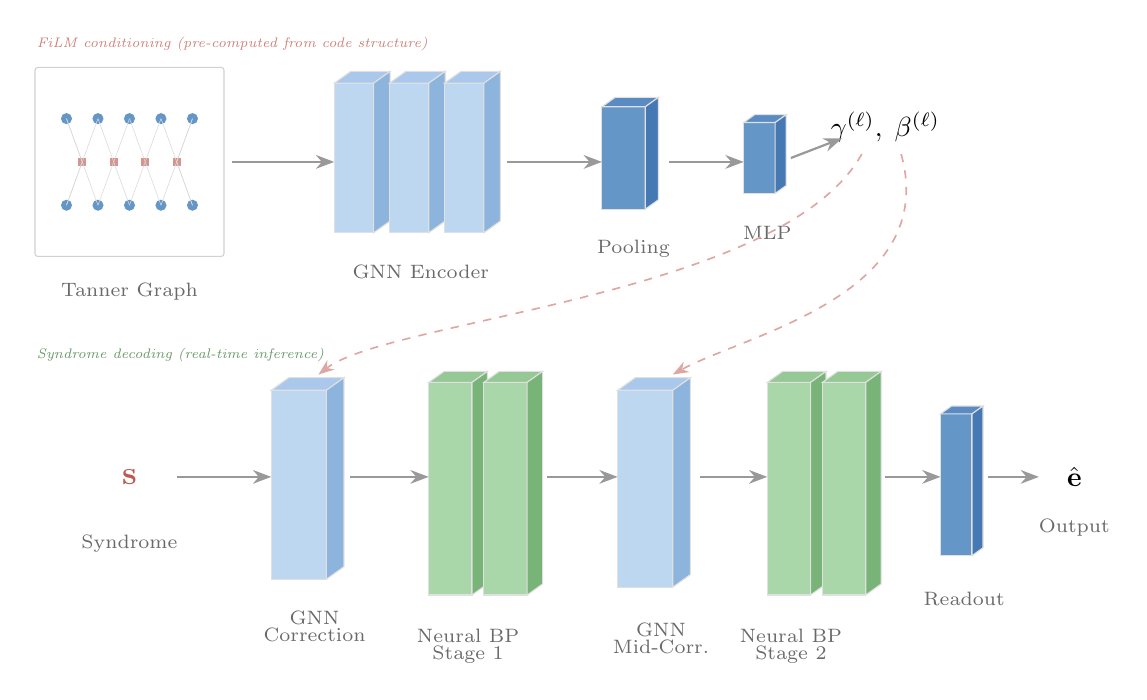
\begin{tikzpicture}[>=Stealth, font=\sffamily]

% ── 3D cuboid: \cub{x}{y}{w}{h}{d}{front}{side}{top} ──
\newcommand{\cub}[8]{%
    \fill[#6] (#1,#2) rectangle ++(#3,#4);
    \draw[black!12] (#1,#2) rectangle ++(#3,#4);
    \fill[#8] (#1,{#2+#4}) -- ++({#5*0.28},{#5*0.20})
        -- ++(#3,0) -- ++({-#5*0.28},{-#5*0.20}) -- cycle;
    \draw[black!12] (#1,{#2+#4}) -- ++({#5*0.28},{#5*0.20})
        -- ++(#3,0) -- ++({-#5*0.28},{-#5*0.20}) -- cycle;
    \fill[#7] ({#1+#3},#2) -- ++({#5*0.28},{#5*0.20})
        -- ++(0,#4) -- ++({-#5*0.28},{-#5*0.20}) -- cycle;
    \draw[black!12] ({#1+#3},#2) -- ++({#5*0.28},{#5*0.20})
        -- ++(0,#4) -- ++({-#5*0.28},{-#5*0.20}) -- cycle;
}

% ════════════════════════════════════════════════
%  TOP ROW — FiLM conditioning path
% ════════════════════════════════════════════════

% Tanner graph (bipartite wireframe)
\begin{scope}[shift={(0,5.0)}]
    \fill[white,opacity=0.45] (0,0) rectangle (2.4,2.4);
    \draw[black!18, rounded corners=1pt] (0,0) rectangle (2.4,2.4);
    % variable nodes
    \foreach \x in {0.4,0.8,1.2,1.6,2.0}{
        \fill[db] (\x,1.75) circle(2pt);
        \fill[db] (\x,0.65) circle(2pt);
    }
    % check nodes
    \foreach \x in {0.6,1.0,1.4,1.8}{
        \fill[rr!55] (\x,1.2) +(-1.5pt,-1.5pt) rectangle +(1.5pt,1.5pt);
    }
    % edges
    \foreach \x in {0.4,0.8,1.2,1.6,2.0}{
        \pgfmathsetmacro{\cl}{max(\x-0.2,0.6)}
        \pgfmathsetmacro{\cr}{min(\x+0.2,1.8)}
        \draw[black!15,very thin] (\x,1.75)--(\cl,1.2);
        \draw[black!15,very thin] (\x,1.75)--(\cr,1.2);
        \draw[black!15,very thin] (\x,0.65)--(\cl,1.2);
        \draw[black!15,very thin] (\x,0.65)--(\cr,1.2);
    }
\end{scope}
\node[font=\scriptsize,gy] at (1.2,4.55) {Tanner Graph};

% GNN message-passing layers (3 cuboids)
\cub{3.8}{5.3}{0.50}{1.9}{0.75}{lb}{mb}{tb}
\cub{4.5}{5.3}{0.50}{1.9}{0.75}{lb}{mb}{tb}
\cub{5.2}{5.3}{0.50}{1.9}{0.75}{lb}{mb}{tb}
\node[font=\scriptsize,gy] at (4.9,4.8) {GNN Encoder};

% Global mean pooling
\cub{7.2}{5.6}{0.55}{1.3}{0.6}{db}{ds}{dt}
\node[font=\scriptsize,gy] at (7.6,5.1) {Pooling};

% MLP head
\cub{9.0}{5.8}{0.40}{0.9}{0.5}{db}{ds}{dt}
\node[font=\scriptsize,gy] at (9.3,5.3) {MLP};

% FiLM output symbols
\node[font=\normalsize] at (10.8,6.65) {$\gamma^{(\ell)},\;\beta^{(\ell)}$};

% Top-row arrows
\draw[->,thick,black!40] (2.5,6.2) -- (3.8,6.2);
\draw[->,thick,black!40] (6.0,6.2) -- (7.2,6.2);
\draw[->,thick,black!40] (8.05,6.2) -- (9.0,6.2);
\draw[->,thick,black!40] (9.6,6.25) -- (10.25,6.5);

% Subtle row label
\node[font=\tiny\itshape,rr!65,anchor=west] at (-0.1,7.7)
    {FiLM conditioning (pre-computed from code structure)};

% ════════════════════════════════════════════════
%  BOTTOM ROW — Real-time decoding pipeline
% ════════════════════════════════════════════════

% Subtle row label
\node[font=\tiny\itshape,mg!85!black,anchor=west] at (-0.1,3.75)
    {Syndrome decoding (real-time inference)};

% Syndrome input
\node[font=\large,rr!85] at (1.2,2.2) {$\mathbf{s}$};
\node[font=\scriptsize,gy] at (1.2,1.35) {Syndrome};

% GNN LLR Correction
\cub{3.0}{0.9}{0.70}{2.4}{0.80}{lb}{mb}{tb}
\node[font=\scriptsize,gy,align=center] at (3.55,0.3)
    {GNN\\[-2pt]Correction};

% Neural BP Stage 1 (2 green cuboids)
\cub{5.0}{0.7}{0.55}{2.7}{0.70}{lg}{mg}{tg}
\cub{5.7}{0.7}{0.55}{2.7}{0.70}{lg}{mg}{tg}
\node[font=\scriptsize,gy,align=center] at (5.5,0.05)
    {Neural BP\\[-2pt]Stage 1};

% GNN Mid-Correction
\cub{7.4}{0.8}{0.70}{2.5}{0.80}{lb}{mb}{tb}
\node[font=\scriptsize,gy,align=center] at (7.95,0.15)
    {GNN\\[-2pt]Mid-Corr.};

% Neural BP Stage 2 (2 green cuboids)
\cub{9.3}{0.7}{0.55}{2.7}{0.70}{lg}{mg}{tg}
\cub{10.0}{0.7}{0.55}{2.7}{0.70}{lg}{mg}{tg}
\node[font=\scriptsize,gy,align=center] at (9.6,0.05)
    {Neural BP\\[-2pt]Stage 2};

% MLP readout
\cub{11.5}{1.2}{0.40}{1.8}{0.50}{db}{ds}{dt}
\node[font=\scriptsize,gy] at (11.8,0.65) {Readout};

% Decoded errors output
\node[font=\normalsize\bfseries] at (13.2,2.2) {$\hat{\mathbf{e}}$};
\node[font=\scriptsize,gy] at (13.2,1.55) {Output};

% Bottom-row arrows
\draw[->,thick,black!40] (1.8,2.2) -- (3.0,2.2);
\draw[->,thick,black!40] (4.0,2.2) -- (5.0,2.2);
\draw[->,thick,black!40] (6.5,2.2) -- (7.4,2.2);
\draw[->,thick,black!40] (8.45,2.2) -- (9.3,2.2);
\draw[->,thick,black!40] (10.8,2.2) -- (11.5,2.2);
\draw[->,thick,black!40] (12.1,2.2) -- (12.75,2.2);

% ════════════════════════════════════════════════
%  FiLM conditioning arrows (dashed, top → bottom GNNs)
% ════════════════════════════════════════════════

\draw[->,dashed,rr!45,semithick]
    (10.5,6.3) .. controls (9.5,4.5) and (4.5,4.2) .. (3.6,3.5);
\draw[->,dashed,rr!45,semithick]
    (11.0,6.3) .. controls (11.5,4.5) and (9.0,4.0) .. (8.1,3.5);

\end{tikzpicture}
\end{document}
